\documentclass[letterpaper]{article}
\usepackage{amsmath}
\usepackage{tikz}
\usepackage{epigraph}
\usepackage{lipsum}
\usepackage{hyperref}
\usepackage{tocloft}
\usepackage{graphicx}
\usepackage{float}

\usepackage{setspace, amsmath}

\usepackage[centering,includeheadfoot,margin=2cm]{geometry}
\usepackage{xcolor}
\usepackage{calc,blindtext}

\renewcommand\epigraphflush{flushright}
\renewcommand\epigraphsize{\normalsize}
\setlength\epigraphwidth{0.6\textwidth}

\definecolor{titlepagecolor}{cmyk}{1,.60,0,.40}

\DeclareFixedFont{\titlefont}{T1}{ppl}{b}{it}{1.0in}

\def\printauthor{%
    {\large \@author}}
\makeatother
\author{%
    Nico Taljaard \\
    10153285 \\%vspace{20pt} \\
    Gerhard Smit \\
    12282945 \\%vspace{20pt} \\
    Martin Schoeman \\
    10651994 \\
}

\begin{document}

\begin{titlepage}

\newcommand{\HRule}{\rule{\linewidth}{0.5mm}} % Defines a new command for the horizontal lines, change thickness here

\begin{center} % Center everything on the page
 
%----------------------------------------------------------------------------------------
%   HEADING SECTIONS
%----------------------------------------------------------------------------------------

%\textsc{\LARGE University Name}\\[1.5cm] % Name of your university/college
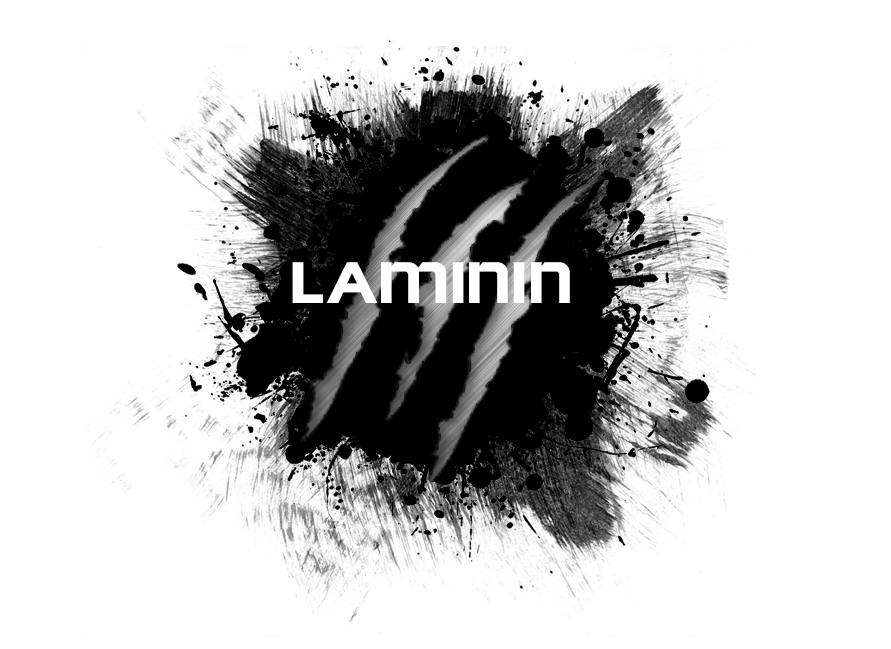
\includegraphics[width=50mm]{laminin.png} \\
\textsc{\Large University of Pretoria}\\[0.2cm] % Major heading such as course name
\textsc{\large Derivco - Rodney Pillay}\\[0.2cm] % Minor heading such as course title

%----------------------------------------------------------------------------------------
%   TITLE SECTION
%----------------------------------------------------------------------------------------

\HRule \\[0.4cm]
{ \huge \bfseries Corpse Slasher by Laminin}\\[0.4cm] % Title of your document
\HRule \\[0.5cm]
 
%----------------------------------------------------------------------------------------
%   AUTHOR SECTION
%----------------------------------------------------------------------------------------

\begin{minipage}{0.4\textwidth}
\begin{flushleft} \large
\emph{COS 301 Software Engineering}\\
\vspace{1cm}
Code Documentation
\end{flushleft}
\end{minipage}
~
\begin{minipage}{0.4\textwidth}
	\begin{flushright} \large
	\emph{Developers:} \\
		%\printauthor % Supervisor's Name
		NJ \textsc{Taljaard} \\
			\begin{small}
				10153285
			\end{small} \\
		M  \textsc{Schoeman} \\
			\begin{small}
				10651994 \\
			\end{small}
		G  \textsc{Smith} \\
			\begin{small}
				12282945
			\end{small}
	\end{flushright}
\end{minipage}\\

% If you don't want a supervisor, uncomment the two lines below and remove the section above
%\Large \emph{Author:}\\
%John \textsc{Smith}\\[3cm] % Your name

%----------------------------------------------------------------------------------------
%   LOGO SECTION
%----------------------------------------------------------------------------------------


\includegraphics[width=60mm, height=80mm]{corpseslasher.png}\\ % Include a department/university logo - this will require the graphicx package
 
%----------------------------------------------------------------------------------------
\end{center}
\vfill % Fill the rest of the page with whitespace

\end{titlepage}

% % % % % % % % % % % % % % %
% 							%
%	Remainder of document	%
% 							%
% % % % % % % % % % % % % % % 

	\newpage
		{\LARGE \bf Change Log}\\[2em]
		
		\begin{tabbing}
			\hspace*{2.5cm}\=\hspace*{2.5cm}\=\hspace*{8cm}\=\hspace*{3cm} \kill
			28/07/2014	\> Version 1.0	\> Document Created 							\> Nico Taljaard \\
			31/07/2014  \> Version 1.1  \> Added code documentation						\> Nico Taljaard\\
			20/08/2014  \> Version 2.0  \> Updated game code documentation				\> Nico Taljaard\\
			22/08/2014  \> Version 2.0  \> Added unit testing code documentation.		\> Martin Schoeman\\
			09/10/2014	\> Version 3.0	\> Updated game code documentation.				\> Nico Taljaard\\
		\end{tabbing}
		
	\newpage
		\renewcommand\contentsname{TABLE OF CONTENTS}
		\newcommand\contentsnameLC{\colorbox{blue}{\makebox[\textwidth-2\fboxsep][l]{\bfseries\color{white} Table of Contents}}}
		
		\renewcommand{\cftdot}{}
		\hypersetup{linktocpage}
		\tableofcontents
		
		\begin{flushleft}
			\LARGE\href{https://github.com/njTaljaard/Laminin_CorpseSlasher/}{Git repository: Laminin - Corpse Slasher}
		\end{flushleft}
		
		\newpage
		
		\section*{\colorbox{blue}{\makebox[\textwidth-2\fboxsep][l]{\bfseries\color{white} Code Documentation }}} \addcontentsline{toc}{section}{Code Documentation}
				\vspace{0.1in}
				
					\subsection*{Game Main:}
					\addcontentsline{toc}{subsection}{Game Main}
					\vspace{0.1in}
						
						\begin{itemize}
							\item 	All Implemented Interfaces: \\
									com.jme3.system.SystemListener, de.lessvoid.nifty.screen.ScreenController
							\item	Field Summary
									\begin{itemize}
										\item	(package private) de.lessvoid.nifty.controls.TextField	accEmail 
										\item	(package private) de.lessvoid.nifty.controls.TextField	accName 
										\item	(package private) de.lessvoid.nifty.controls.TextField	accPassword 
										\item	(package private) de.lessvoid.nifty.controls.TextField	accPasswordRE 
										\item	(package private) de.lessvoid.nifty.controls.TextField	accSurname 
										\item	(package private) de.lessvoid.nifty.controls.TextField	accUser 
										\item	(package private) com.jme3.bullet.BulletAppState	bulletAppState 
										\item	(package private) static int	byPass 
										\item	(package private) GameScene	gameScene 
										\item	(package private) boolean	loggedIn 
										\item	(package private) de.lessvoid.nifty.controls.TextField	passwordTxt 
										\item	(package private) de.lessvoid.nifty.elements.Element	progressBarElement 
										\item	(package private) de.lessvoid.nifty.controls.TextField	retUser 
										\item	(package private) de.lessvoid.nifty.controls.RadioButtonGroupStateChangedEvent	selectedButton 
										\item	(package private) de.lessvoid.nifty.elements.render.TextRenderer	textRenderer 
										\item	(package private) jme3utilities.TimeOfDay	timeOfDay 
										\item	(package private) UserInterfaceManager	UI 
										\item	(package private) de.lessvoid.nifty.controls.TextField
									\end{itemize} 
							\item	Fields inherited from class com.jme3.app.SimpleApplication \\
									flyCam, fpsText, guiFont, guiNode, INPUT\_MAPPING\_CAMERA\_POS, \\ INPUT\_MAPPING\_EXIT, INPUT\_MAPPING\_HIDE\_STATS, INPUT\_MAPPING\_MEMORY, \\ rootNode, showSettings
							\item	Fields inherited from class com.jme3.app.Application \\
									assetManager, audioRenderer, cam, context, guiViewPort, inputEnabled, inputManager, joyInput, keyInput, listener, mouseInput, paused, pauseOnFocus, renderer, renderManager, settings, speed, stateManager, timer, touchInput, viewPort
							\item	Constructor Summary \\
									Main()
							\item	Methods inherited from class com.jme3.app.SimpleApplication \\
									getFlyByCamera, getGuiNode, getRootNode, initialize, isShowSettings, loadGuiFont, setDisplayFps, setDisplayStatView, setShowSettings, start, update
							\item	Methods inherited from class com.jme3.app.Application \\
									createCanvas, destroy, destroyInput, enqueue, gainFocus, getAssetManager, getAudioRenderer, getCamera, getContext, getGuiViewPort, getInputManager, getListener, getRenderer, getRenderManager, getStateManager, getTimer, getViewPort, handleError, isPauseOnLostFocus, loseFocus, requestClose, reshape, restart, runQueuedTasks, setAssetManager, setPauseOnLostFocus, setSettings, setTimer, start, startCanvas, startCanvas, stop, stop
							\item	Method Detail
									\begin{itemize}
										\item	main \\
												public static void main(java.lang.String[] args)
										\item	simpleInitApp \\
												public void simpleInitApp() \\ \\
												This function only gets called once. Use this function to create the login screen where after the scene will be compiled during loading screen. \\ \\
												Specified by: \\
												simpleInitApp in class com.jme3.app.SimpleApplication
										\item	simpleUpdate \\
												public void simpleUpdate(float tpf) \\ \\
												Overrides: \\
												simpleUpdate in class com.jme3.app.SimpleApplication
										\item	simpleRender \\
												public void simpleRender(com.jme3.renderer.RenderManager rm) \\ \\
												Overrides: \\
												simpleRender in class com.jme3.app.SimpleApplication
										\item	loadSettings
												public boolean[] loadSettings() \\ \\
												Returns: \\
												an array of booleans checking which settings to activate. Loading the settings based on the .txt file
										\item	loadGame \\
												public void loadGame() \\ \\
												This function assembles all the game elements in order to render the game.
										\item	bind \\
												public void bind(de.lessvoid.nifty.Nifty nifty,de.lessvoid.nifty.screen.Screen screen) \\ \\
												Specified by:
												bind in interface de.lessvoid.nifty.screen.ScreenController \\ \\
												Parameters:
												nifty - the object containing all the components of the GUI \\
												screen - the actual screen panel of the nifty GUI at the binding of the create \\ account screen all the appropriate text field's data are collected and checked
										\item	onStartScreen \\
												public void onStartScreen() \\ \\
												Specified by: \\
												onStartScreen in interface de.lessvoid.nifty.screen.ScreenController
										\item	onEndScreen \\
												public void onEndScreen() \\ \\
												Specified by: \\
												onEndScreen in interface de.lessvoid.nifty.screen.ScreenController
										\item	radioButtons \\
												public void radioButtons(java.lang.String id, de.lessvoid.nifty.controls.RadioButtonGroupStateChangedEvent event) \\ \\
												Parameters: \\
												id - the ID of radio button selected \\
												event - the state of the selected radio button on a state change the button event is updated
										\item	loadingScreen
												public void loadingScreen() \\ \\
												After a successful login the loading screen is loaded and the game starts to load
										\item	newAccount \\
												public void newAccount() \\ \\
												Changes the screen to the new account screen
										\item	createNewAccount \\
												public void createNewAccount() \\ \\
												Checks all the appropriate fields whther they are valid and then adds the data to the database and logins in
										\item	retrievePassword \\
												public void retrievePassword() \\ \\
												Goes to the retrieve password screen
										\item	loginScreen \\
												public void loginScreen() \\
												Goes to the login screen
										\item	quitGame \\
												public void quitGame() \\ \\
												Quits the game
										\item	graphicsScreen \\
												public void graphicsScreen() \\ \\
												Goes to the graphics settings from the option screen
										\item	audioScreen \\
												public void audioScreen() \\ \\
												Goes to the audio settings from the option screen
										\item	difficultyScreen
												public void difficultyScreen() \\ \\
												Goes to the difficulty settings from the option screen
										\item	goBack \\
												public void goBack() \\ \\
												Goes back to the login screen
										\item	socialLogin \\
												public void socialLogin(java.lang.String type) \\ \\
												Logins in via the selected social media
									\end{itemize}
						\end{itemize}
						
					\vspace{0.2in}
					\subsection*{Game documentation:}
					\addcontentsline{toc}{subsection}{Game documentation}
					\vspace{0.1in}
					
						\subsubsection*{GameScene:}
						\addcontentsline{toc}{subsubsection}{GameScene}
						\vspace{0.1in}
							\begin{itemize}
								\item	Field Summary
										\begin{itemize}
											\item	private BasicScene	basicScene 
											\item	private Character	character 
											\item	private CollisionController	collController 
											\item	private MobsHandler	mobHandler 
											\item	private java.util.ArrayList<java.lang.String>	mobHits 
											\item	private boolean	playerAttacking 
											\item	private com.jme3.scene.Node	sceneNode 
										\end{itemize}
								\item	Constructor Detail \\
										public GameScene(int selectedMap, com.jme3.asset.AssetManager assestManager,\\
										         com.jme3.renderer.ViewPort viewPort,
										         com.jme3.renderer.Camera cam, \\
										         com.jme3.bullet.BulletAppState bullet,
										         com.jme3.input.InputManager inMan) \\ \\
										GameScene will combine all the entities of the entire game into a node for a reverance point for the game engine. \\ \\
										Parameters: \\
										selectedMap - - the desired map to load. \\
										assetManager - - Assetmanager passed through from main game. \\
										viewPort - - ViewPort required for water, contains position of camara. \\
										cam - - Camera to assign to player and mouse motion.
								\item	Method Detail
										\begin{itemize}
											\item	reloadScene() \\
													reloadScene - After graphic settings was changed. \\
											\item	relog \\
													relog(com.jme3.renderer.Camera cam, int selectedMap) \\ \\
													relog - After game was logged out and back in to reset to starting position. \\ \\
													Parameters: \\
													cam - - Replace player. \\
													selectedMap - - Determine camera location. \\
											\item	initScene \\
													private void initScene(com.jme3.renderer.ViewPort viewPort,
													             com.jme3.renderer.Camera cam, \\
													             int map) \\ \\
													initScene will retrieve and combine all the variase assets that will make up the entire scene. \\ \\
													Parameters: \\
													viewPort - - ViewPort required for post processing filter: Water. \\
													cam - - Camera required for the sky controller to update the postion of assets. \\
													map - - Corresponding scene number to assign the required terrain. \\
											\item	initMainCharacter \\
													private void initMainCharacter(com.jme3.input.InputManager inMan, \\
													                     com.jme3.renderer.Camera cam) \\ \\
													initMainCharacter will load the main player model, add it to a character handler to be able to add gravity and move it around, also add the key and mouse functionality to control and update it the model and camera positions. \\ \\
													Parameters: \\
													inMan - - InputManager for adding key and mouse binding to be triggered. \\
													cam - - Camera to be bound to player model.\\
											\item	initMobs \\
													private void initMobs() \\ \\
													initMobs will be responsible for creating all the mobs at specified positions also update its position, animation and aggression control. \\ \\
											\item	initCameraPosition \\
													private void initCameraPosition(com.jme3.renderer.Camera cam, \\
				                      int map) \\ \\
													initCameraPosition will be used the multiple maps are create to define the correct camera position. \\ \\
													Parameters: \\
													cam - - Camera from main game. \\
													map - - The scene to be loaded. \\
											\item	initAudio \\
													private void initAudio() \\ \\
													initAudio - Loads all audio nodes required. \\ \\
											\item	update \\
													public void update(jme3utilities.TimeOfDay tod, \\
				          float tpf) \\ \\
													update will update the all the corrisponding assets of the game. From light direction, time of day, water light reflection, character position. \\ \\
													Parameters: \\
													tod - - TimeOfDay to update the skycontrol time of day. \\
													tpf - - Update value of time between frames. \\
											\item	retrieveSceneNode \\
													public com.jme3.scene.Node retrieveSceneNode() \\ \\
													retrieveSceneNode to obtain the node that contains all the assests of the scene which will be added to the rootNode for it to be renderable. \\
													Returns: \\
													sceneNode consisting of the entire scene.
										\end{itemize}
							\end{itemize}
						
						\vspace{0.2in}
						\subsubsection*{BasicScene:}
						\addcontentsline{toc}{subsubsection}{BasicScene}
						\vspace{0.1in}
							\begin{itemize}
								\item	Field Summary
										\begin{itemize}
											\item	private com.jme3.light.AmbientLight	ambient 
											\item	private com.jme3.renderer.Camera	cam 
											\item	private com.jme3.post.FilterPostProcessor	fpp 
											\item	private com.jme3.math.Vector3f	lightDir 
											\item	private com.jme3.water.WaterFilter	postWater 
											\item	private com.jme3.scene.Node	sceneModel
											\item	private java.lang.String	sceneName 
											\item	private com.jme3.scene.Node	sceneNode 
											\item	private com.jme3.water.SimpleWaterProcessor	simpleWater 
											\item	private com.jme3.scene.Spatial	skybox 
											\item	private jme3utilities.sky.SkyControl	skyControl 
											\item	private com.jme3.light.DirectionalLight	sun 
											\item	private com.jme3.renderer.ViewPort	vp 
										\end{itemize}
								\item	Constructor Detail \\
										public BasicScene(java.lang.String mapName) \\ \\
										BasicScene will create the scene attached to sceneNode. \\ \\
										Parameters: \\
										mapName - - Map that you desire to load.
								\item	Method Detail
										\begin{itemize}
											\item	createScene \\
													public void createScene(com.jme3.renderer.ViewPort vp,
													               com.jme3.renderer.Camera cam) \\ \\
													createScene will call the appopriate functions to create the scene and attached it to sceneNode, which will be added to rootNode higher up to be able to draw. \\ \\
													Parameters: \\
													vp - - ViewPort required for water, contains position of camara. \\
													cam - - Camera required to create a day night skybox system. \\
											\item	reloadScene \\
													public void reloadScene() \\ \\
													reloadScene - Called after graphics settings have been changed and applied.
											\item	initAmbientLight \\
													private void initAmbientLight() \\ \\
													initAmbientLight will crreate the basic ambient light to be able to see within the scene. \\
											\item	initSunLight \\
													private void initSunLight() \\ \\
													initSunLight will create the scenes sunlight with a given direction and color.
											\item	initTerrain \\
													private void initTerrain() \\
													initTerrain - will load the Scene j3o for the appropriate scene and attach it to the basic scene node, which contains the terrain, trees and camp site. Add collision detection to all object to create a realistic scene. \\
											\item	initWater \\
													private void initWater() \\ \\
													initWater will determine which water needs to be load from settings.
											\item	initBasicWater \\
													private void initBasicWater() \\ \\
													initBasicWater will create a low performance water system consisting of basic movement and reflection no post processing. \\
											\item	initPostProcessWater \\
													private void initPostProcessWater() \\ \\
													initWater will create a per pixel motion water quad and add it to the scene. To be used by the higher end system. \\
											\item	initSkyBox \\
													private void initSkyBox() \\ \\ 
													initSkyBox will determine which skybox needs to be load from settings. \\
											\item	initBasicSky \\
													private void initSkyBox() \\ \\ 
													initBasicSky will create a basic skybox consisting of a cube with textures. \\
											\item	initSkyControl \\
													private void initSkyControl() \\ \\ 
													initSkyControl will create a day night system skybox consisting of a moving sun and moon, a rotating star system and a changing day night sky. \\
											\item	update \\
													public void update(jme3utilities.TimeOfDay tod,
				          float tpf) \\ \\
													Update basic scene between frame. \\ \\
													Parameters: \\
													tod - - Time within the world. \\
													tpf - - Time between frames. \\
											\item	retrieveSceneNode \\
													public com.jme3.scene.Node retrieveSceneNode() \\ \\
													Returns: \\
													the basic scene node to be added to the game node.
										\end{itemize}
							\end{itemize}
						
						\vspace{0.2in}
						\subsubsection*{Character:}
						\addcontentsline{toc}{subsubsection}{Character}
						\vspace{0.1in}
						
							\begin{itemize}
								\item	Field Summary
										\begin{itemize}
											\item	protected static boolean	aggro 
											\item	protected static boolean	alive 
											\item	protected static com.jme3.asset.AssetManager	assetManager 
											\item	protected static com.jme3.bullet.BulletAppState	bullet 
											\item	static int	dialogInterval 
											\item	static int	dialogPlayed 
											\item	static float	eighth\_pi 
											\item	static int	hitSplahsInterval 
											\item	static int	hitSplash 
											\item	static int	mobRegenInterval 
											\item	static int	mobRespawnTimer 
											\item	static float	mobRunSpeed 
											\item	static float	mobWalkSpeed 
											\item	static float	playerCameraXSpeed 
											\item	static float	playerCameraYSpeed 
											\item	protected static com.jme3.math.Vector3f	playerPosition 
											\item	static int	playerRegenInterval 
											\item	static int	playerRespwanTime 
											\item	static float	playerWalkSpeed 
											\item	static java.util.Random	rand 
											\item	static int	systemTime 
										\end{itemize}
								\item	Constructor Detail \\
										public GameWorld() \\ \\
								\item	Method Detail \\
										\begin{itemize}
											\item	getSkeletonControl \\
													public static com.jme3.animation.SkeletonControl \\ getSkeletonControl(com.jme3.scene.Node model) \\ \\
													getSkeletonControl - Recursive search to find a skeleton controller of the required model. \\ \\
													Parameters: \\
													model - - Model to be searched. \\
													Returns: \\
													SkeletonControl of model if found.
											\item	getAnimationControl \\
													public static com.jme3.animation.AnimControl getAnimationControl(com.jme3.scene.Node model) \\ \\
													getAnimCOntrol - Recursive search to find an animation controller of the required model. \\ \\
													Parameters: \\
													model - - Model to be searched. \\
													Returns: \\
													AnimControl of model if found. \\
											\item	getLookAt \\
													public static com.jme3.math.Vector3f getLookAt() \\ \\
													getLookAt - Generates a random direction for a mob to look at, at spawn, respawn and aggro loss. \\ \\
													Returns: \\
													lookAt - Vector3f to set lookAt of model. \\
											\item	getNextGaussian \\
													public static float getNextGaussian(int range) \\ \\
													getNextGaussian - Generates a random value from Random. \\ \
													Parameters: \\
													range - - The range to create a value within. \\
													Returns: \\
													random number - float. \\
											\item	updateAggro \\
													public static void updateAggro(boolean agg) \\ \\
													updateAggro - During mob concurrent update each mob updates its own aggro state to set overall aggro to true is so. \\ \\
													Parameters: \\
													agg - - Mob aggro state. \\
											\item	removeAggro \\
													public static void removeAggro() \\ \\
													removeAggro - Player removes aggro after update, mobs update after. \\
											\item	setAlive \\
													public static void setAlive(boolean alv) \\ \\
													setAlive - Player updates alive or death at each update. \\ \\
													Parameters: \\
													alv - - Players alive state.
											\item	setPlayerPosition \\
													public static void setPlayerPosition(com.jme3.math.Vector3f vec) \\ \\
													setPlayerPosition - Player updates its current position at each udpate. \\ \\
													Parameters: \\
													vec - - Player position.
										\end{itemize}
							\end{itemize}
						
						\vspace{0.2in}
						\subsubsection*{Character:}
						\addcontentsline{toc}{subsubsection}{Character}
						\vspace{0.1in}
							\begin{itemize}
								\item	Field Summary
										\begin{itemize}
											\item	private CharacterAnimControl	animController 
											\item	private com.jme3.renderer.Camera	cam 
											\item	private CharacterCameraControl	cameraController 
											\item	private com.jme3.animation.AnimChannel	channel 
											\item	private com.jme3.bullet.control.BetterCharacterControl	characterControl 
											\item	private com.jme3.animation.AnimControl	control 
											\item	private int	deathTime 
											\item	private float	health 
											\item	private CharacterMotionControl	motionController 
											\item	private com.jme3.scene.Node	player 
											\item	private com.jme3.scene.Node	playerNode 
											\item	private ModelRagdoll	ragdoll 
											\item	private int	regenTime 
											\item	private com.jme3.bullet.control.GhostControl	swordControl 
											\item	private com.jme3.math.Vector3f	walkDirection  
										\end{itemize}
								\item	Constructor Detail \\
										public Character(com.jme3.input.InputManager inMan, \\
		        com.jme3.renderer.Camera cam) \\ \\
										Character will consist of loading the model with its materials and rigging, add physics to the model and bind the camera to the model. \\ \\
										Parameters: \\ \\
										inMan - - InputManager required to set up key bindings. \\
										cam - - Camera use for camera movement and attacking the player model to move with camera. \\
								\item	Method Detail 
										\begin{itemize}
											\item	initModel \\
													private void initModel() \\ \\
													initModel loads the model and sets it to the specified position. \\
											\item	initControl \\
													private void initControl() \\ \\
													initControl sets up the character controller responsible for collision, motion and forces control.
											\item	initSwordGhost \\
													private void initSwordGhost() \\ \\
													initSwordGhost sets up the collision box that will be bound to the players sword in order to determine if any collision has occured with the sword and a mob.
											\item	initRagdoll \\
													private void initRagdoll() \\
											\item	assemblePlayer \\
													private void assemblePlayer() \\ \\
													assemblePlayer add the controllers to the player and to the physics handler. \\
											\item	initCamera \\
													private void initCamera() \\ \\
													initCamera will attach the camera to the player for motion control. \\
											\item	initAnim \\
													private void initAnim() \\ \\
													initAnim creates the controller and animations channel required to access all available animations, set the current animation and the type of trigger at the end of a animations cycle.
											\item	updateCharacterPostion \\
													public boolean updateCharacterPostion(int playerHits,
													                             float tpf) \\ \\
													updateCharacterPosition will be called from the main game update function on every frame update, where this will call the motion and animation updater separetly. \\ \\
													Parameters: \\
													playerHits - - number of mobs hit, to check if player is currently in an attacking position. \\
													tpf - - Time per frame to update ragdoll position. \\
											\item	processKnocks \\
													public void processKnocks(java.util.ArrayList<java.lang.String> knocks) \\ \\
													processKnocks will process all the landed attacks from mobs. \\ \\
													Parameters: \\
													knocks - - ArraysList of mob names that have hit player. \\
											\item	swapControllers \\
													private void swapControllers() \\ \\
													swapControllers will swap between controllers from BetterCharacterControl will ghost boxes for alive and ragdoll for death. \\
											\item	initKeys \\
													private void initKeys(com.jme3.input.InputManager inMan) \\
													initKeys sets up the key bindings that will be used to control the player model. \\ \\
													Parameters: \\
													inMan - - InputManager add all the required key mappings to be triggered when pressed.
											\item	retrievePlayerNode \\
													public com.jme3.scene.Node retrievePlayerNode() \\ \\
													retrievePlayerNode an accessor to the game node containing the player model. \\ \\
													Returns: \\
													playernode - Node containing the model data.
										\end{itemize}
							\end{itemize}
						
						\vspace{0.2in}
						\subsubsection*{CharacterMotionControl:}
						\addcontentsline{toc}{subsubsection}{CharacterMotionControl}
						\vspace{0.1in}
							\begin{itemize}
								\item	Field Summary
										\begin{itemize}
											\item	private com.jme3.input.controls.ActionListener	actionListener 
											\item	private com.jme3.renderer.Camera	cam 
											\item	private boolean	down 
											\item	protected boolean	jump 
											\item	private boolean	left 
											\item	private boolean	right 
											\item	protected boolean	slash 
											\item	private boolean	up 
											\item	protected boolean	walk 
											\item	private com.jme3.math.Vector3f	walkDirection  
										\end{itemize}
								\item	Constructor Detail \\
										public CharacterMotionControl() \\ \\
										CharacterMotionControl will set all the values and initialize the Action Listener for the key bindings.
								\item	Method Detail 
										\begin{itemize}
											\item	initMotionController \\
													private void initMotionController() \\ \\
													initMotionController will create the Action Listener which will trigger when a butten is pressed and released, updating the corrisponding values to be able to calulate the resulting motion and required animation.
											\item	updateCharacterMotion \\
													public com.jme3.math.Vector3f updateCharacterMotion(com.jme3.renderer.Camera cam) \\ \\
													updateCharacterMotion will calulate the resulting directional vector from the keys pressed. \\ \\
													Parameters: \\
													cam - - Camera required for the camera directional and left vector. \\ \\
													Returns: \\ 
													walkDirection - The vector containing the new direction and magnatude of the motion.
											\item	getMotionController \\
													public com.jme3.input.controls.ActionListener getMotionController() \\ \\
													getMotionController is the accessor for the motion Action Listener. \\ \\
													Returns: \\
													actionListener.
										\end{itemize}
							\end{itemize}
						
						\vspace{0.2in}
						\subsubsection*{CharacterCameraControl:}
						\addcontentsline{toc}{subsubsection}{CharacterCameraControl}
						\vspace{0.1in}
							\begin{itemize}
								\item	Field Summary
										\begin{itemize}
											\item	private com.jme3.input.controls.AnalogListener	analogListener 
											\item	private com.jme3.scene.CameraNode	cameraNode 
											\item	private com.jme3.bullet.control.BetterCharacterControl	characterControl 
											\item	private float	maxVerticalAngle 
											\item	private float	minVerticalAngle 
											\item	private com.jme3.scene.Node	pivot 
											\item	private float	verticalAngle 
											\item	private float	xMovementSpeed 
											\item	private float	yMovementSpeed
										\end{itemize}
								\item	Constructor Detail \\
										public CharacterCameraControl(java.lang.String name, \\
		                     com.jme3.renderer.Camera cam, \\
		                     com.jme3.scene.Node player, \\
		                     com.jme3.bullet.control.BetterCharacterControl cc) \\ \\
										CharacterCameraControl will create the functionality that will enable the user to move the camera left and right. \\ \\
										Parameters: \\
										name - - Name of camera node. \\
										cam - - Camera as to add to the camera node to control the camera. \\
										player - - Spatial node containing the model and all its controllers.
								\item	Method Detail
										\begin{itemize}
											\item	initActionListener \\
													private void initActionListener() \\ \\
													initActionListener to update the mouse motion.
											\item	verticalRotate \\
													public void verticalRotate(float angle) \\ \\
													verticalRotate will update the vertical rotation of the camera according to the maximum and minimum rotation specified. \\ \\
													Parameters: \\
													angle - - Mouse motion converted to an angle to update the direction.
											\item	getAnalogListener \\
													public com.jme3.input.controls.AnalogListener getAnalogListener() \\ \\
													getAnalogListener is the accessor for the mouse motion Analog Listener. \\ \\
													Returns: \\
													analogListener.
										\end{itemize}
							\end{itemize}
						
						\vspace{0.2in}
						\subsubsection*{CharacterAnimControl:}
						\addcontentsline{toc}{subsubsection}{CharacterAnimControl}
						\vspace{0.1in}
							\begin{itemize}
								\item	Field Summary 
										\begin{itemize}
											\item 	private com.jme3.animation.AnimEventListener	animationListener
										\end{itemize}
								\item	Constructor Detail \\
										public CharacterAnimControl() \\ \\
										CharacterAnimControl will initailize the animation event listener.
								\item	Method Detail
										\begin{itemize}
											\item	initAnimEventListener \\
													private void initAnimEventListener() \\ \\
													initAminEventListener will trigger on animation change as well as when a cycle of an animations if completed to run it again.
											\item	updateCharacterAnimations \\
													public boolean updateCharacterAnimations(com.jme3.animation.AnimChannel channel, \\
				                                boolean slash, \\
				                                boolean walk) \\ \\
													handleAnimations updates animations where required. \\ \\
													Parameters: \\
													channel - - AnimChannel controls the animation currently being used. \\
													slash - - If player is attacking. \\
													walk - - If player is currently walking. \\
											\item	getAnimationListener \\
													public com.jme3.animation.AnimEventListener getAnimationListener() \\ \\
													getAnimationListener accessor of the animation handler. \\ \\
													Returns: \\
													AnimEventListener
										\end{itemize}
							\end{itemize}
						
						\vspace{0.2in}
						\subsubsection*{MobsHandler:}
						\addcontentsline{toc}{subsubsection}{MobsHandler}
						\vspace{0.1in}
							\begin{itemize}
								\item	Field Summary
										\begin{itemize}
											\item	private java.util.ArrayList<java.lang.String>	landedAttacks 
											\item	private com.jme3.scene.Node	mobNode 
											\item	private java.util.ArrayList<Mob>	mobs 
											\item	private java.util.ArrayList<com.jme3.math.Vector3f>	positions 
											\item	private java.util.concurrent.ExecutorService	threadExecutors 
										\end{itemize}
								\item	Constructor Detail
										public MobsHandler(n) \\ \\
										MobHandler will be in control of create mobs at the predefined positions. \\ \\
								\item	Method Detail
										\begin{itemize}
											\item	initPositions \\
													private void initPositions() \\ \\
													initPositions initialize a list of positions where mobs are to be spawned.
											\item	createMobs \\
													private void createMobs() \\ \\
													createMobs creates each mob and adds it to the list of mobs as well as the scene node. \\
											\item	updateMobs \\
													public java.util.ArrayList<java.lang.String> updateMobs(java.util.ArrayList<java.lang.String> playerHits,
													java.util.ArrayList<java.lang.Integer> mobHits,
													float tpf) \\ \\
													updateMobs will update each of the mobs individually. \\ \\
													Parameters: \\
													playerHits - - ArrayList containing the mob name that player has hit. \\
													mobHits - - Collision groups of mobs that have hit player. \\
													tpf - - Time per frame to update ragdoll. \\
											\item	retrieveMobs \\
													public com.jme3.scene.Node retrieveMobs() \\ \\
													retrieveMobs to attach all mobs to rootNode. \\ \\
													Returns: \\
													mobNode - Node contains all the mobs in the scene.
										\end{itemize}
							\end{itemize}
						
						\vspace{0.2in}
						\subsubsection*{Mob:}
						\addcontentsline{toc}{subsubsection}{Mob}
						\vspace{0.1in}
							\begin{itemize}
								\item 	extends java.lang.Thread\\
										All implemented interface: \\
										java.lang.Runnable \\	
								\item	Field Summary
										\begin{itemize}
											\item	private boolean	alive 
											\item	private MobAnimControl	animControl 
											\item	protected boolean	attackAudio 
											\item	private com.jme3.bullet.control.GhostControl	attackGhost 
											\item	protected java.lang.String	attackLanded 
											\item	private com.jme3.animation.AnimChannel	channel 
											\item	private com.jme3.bullet.control.BetterCharacterControl	characterControl 
											\item	private com.jme3.animation.AnimControl	control 
											\item	protected boolean	damageAudio 
											\item	private int	deathTime 
											\item	protected int	handColliosionGroup 
											\item	private float	health 
											\item	private com.jme3.scene.Node	mob 
											\item	private boolean	mobHit 
											\item	protected java.lang.String	mobName 
											\item	private MobMotionControl	motionControl 
											\item	private com.jme3.math.Vector3f	passivePosition 
											\item	private boolean	playerHit 
											\item	private ModelRagdoll	ragdoll 
											\item	private int	regenTime 
											\item	protected boolean	swapControllers 
											\item	private float	tpf 
											\item	protected boolean	walkAudio 
										\end{itemize}
								\item	Constructor Detail \\
										public Mob(com.jme3.math.Vector3f position, java.lang.String mName) \\ \\ 
										Mob creates a basic mob the required functionality. \\ \\
										Parameters: \\
										position - - Vector3f the position to place the mob at. \\
										mName - - String that defines the name assosiated to this mob required for collision detection.
								\item	Method Detail
										\begin{itemize}
											\item	initMob \\
													private void initMob() \\ \\
													initMob will load the required asset, set it to the required position and name it acordingly. \\ 
											\item	initControl \\
													private void initControl() \\ \\
													initControl creates the character controller responsible for collision, motion and forces control.
											\item	initRagdoll \\
													private void initRagdoll() \\ \\
													initRagdoll - will create the ragdoll required for death animation and assign the required limbs.
											\item	initAttackGhost \\
													private void initAttackGhost() \\ \\
													initAttackGhost sets up the collision box that will be bound to the mobs arm in order to determine if any collision has occured with the hand and the player.
											\item	assembleMob \\
													private void assembleMob() \\
													assembleMob add the controllers to the mob and to the physics handler. \\
											\item	initAnim \\
													private void initAnim() \\ \\
													initAnim creates the controller and animations channel required to access all available animations, set the current animation and the type of trigger at the end of a animations cycle.
											\item	set \\
													public void set(boolean playerHit, boolean mobHit, float tpf) \\ \\
													set - From MobsHandler these values are set before the mob thread is sent of for update. \\ \\
													Parameters: \\
													point - - Vector3f the direction of the player required in the attack phase to move the mobs towards the player. \\
													playerHit - - boolean if the player hit this mob. \\
													mobHit - - boolean if mob has attacked player. \\
													tpf - - Time per frame required for updating ragdoll.
											\item	run \\
													public void run() \\ \\
													updateMob will update the mobs phase according to if aggro was triggers and animations that is required for that phase. \\ \\
													Specified by: \\
													run in interface java.lang.Runnable \\
													Overrides: \\
													run in class java.lang.Thread \\
											\item	swapControllers \\
													private void swapControllers() \\ \\
													swapControllers will swap between controllers from BetterCharacterControl will ghost boxes for alive and ragdoll for death. \\
											\item	getPosition \\
													public com.jme3.math.Vector3f getPosition() \\ \\
													getPosition - Accessor to mobs current position. \\ \\
													Returns: \\
													Vector3f mob position.
											\item	alive \\
													public boolean isAlive() \\ \\
													alive - Accessor to mobs alive state. \\ \\
													Returns: \\
													boolean of mobs alive state. \\
											\item	retrieveMob \\
													public com.jme3.scene.Node retrieveMob() \\ \\
													retrieveMob to access the node containing the single mob. \\ \\
													Returns: \\
													mob - Node this mob.
										\end{itemize}
							\end{itemize}
							
						\vspace{0.2in}
						\subsubsection*{MobAnimControl:}
						\addcontentsline{toc}{subsubsection}{MobAnimControl}
						\vspace{0.1in}	
							\begin{itemize}
								\item	Field Summary
										\begin{itemize}
											\item	private com.jme3.animation.AnimEventListener	animationListener	
										\end{itemize}
								\item	Constructor Detail \\
										public MobAnimControl() \\ \\
								\item	Method Detail
										\begin{itemize}
											\item	initAnimEventListener
													private void initAnimEventListener() \\ \\
													initAminEventListener will trigger on animation change as well as when a cycle of an animations if completed to run it again.
											\item	updateMobAnimations \\
													public void updateMobAnimations(com.jme3.animation.AnimChannel channel, \\
				                       boolean aggro, \\
				                       boolean walkAttack, \\
				                       boolean attack, \\
				                       boolean passive) \\ \\
													updateCharacterAnimations updates animations when required. \\ \\
													Parameters: \\
													channel - - AnimChannel to change and read current animations. \\
													aggro - - Boolean if mob has been aggroed by the player. \\
													walkAttack - - Boolean if mob should attack while walking. \\
													attack - - Boolean if mob can be stationary and attack. \\
													passive - - Boolean if mob is not aggroed and at spawn position.
											\item	getAnimationListener \\
													public com.jme3.animation.AnimEventListener getAnimationListener() \\ \\
													getAnimationListener accessor of the animation handler. \\ \\
													Returns: \\
													AnimEventListener
										\end{itemize}
							\end{itemize}
							
						\vspace{0.2in}
						\subsubsection*{MobMotionControl:}
						\addcontentsline{toc}{subsubsection}{MobMotionControl}
						\vspace{0.1in}	
							\begin{itemize}
								\item	Field Summary
										\begin{itemize}
											\item	protected boolean	aggro 
											\item	private com.jme3.bullet.control.GhostControl	aggroGhost 
											\item	protected boolean	alive 
											\item	protected boolean	attack 
											\item	private float	distanceFromPlayer 
											\item	private float	distanceToPassive 
											\item	private com.jme3.math.Vector3f	motionDirection 
											\item	protected boolean	passive 
											\item	protected boolean	walk 
											\item	protected boolean	walkAttack  
										\end{itemize}
								\item	Constructor Detail \\
										public MobCollisionControl() \\ \\ 
										MobMotionControl - initializes all required variables. \\
								\item	Method Detail
										\begin{itemize}
											\item	initGhost \\
													private void initGhost() \\ \\
													initGhost creates the GhostControl collision sphere that will double as the player detection bounds for changing to attack phase. Also sets the collision group and the group it does collid with.
											\item	updateMobPhase \\
													protected void updateMobPhase(com.jme3.bullet.control.BetterCharacterControl \\ characterControl, com.jme3.math.Vector3f passivePosition, \\
													com.jme3.math.Vector3f mobPosition) \\ \\
													updateMobPhase will determine in which phase the mob is: attack, return, passive. Update the mobs actions to its position and animation. \\ \\
													Parameters: \\
													characterControl - - BetterCharacterControl, model controller of mob
													passivePosition - - Vector3f postion where mob spawn point is. \\
													mobPosition - - Vector3f of mobs current position.
											\item	getAggroGhost \\
													public com.jme3.bullet.control.GhostControl getAggroGhost() \\ \\
													getAggroGhost gives access to the aggro ghost controller. \\ \\
													Returns: \\
													aggoGhost - GhostCollisionBox. \\
											\item	death \\
													public void death(com.jme3.bullet.control.BetterCharacterControl characterControl) \\ \\
													death will turn of motion control so that mob will remain dead. \\ \\
													Parameters: \\
													characterControl - - BetterCharacterControl of mob. \\
										\end{itemize}
							\end{itemize}
							
							\vspace{0.2in}
							\subsubsection*{CollisionController:}
							\addcontentsline{toc}{subsubsection}{CollisionController}
							\vspace{0.1in}	
								\begin{itemize}
									\item	Field Summary
											\begin{itemize}
												\item	private java.util.ArrayList<java.lang.Integer>	mobHits 
												\item	private java.util.ArrayList<java.lang.String>	playerHits 
											\end{itemize}
									\item	Constructor Detail \\
											public CollisionController() \\ \\ \\
									\item	Method Detail
											\begin{itemize}
												\item	collision \\
														public void collision(com.jme3.bullet.collision.PhysicsCollisionEvent event) \\
														collisio processes every collision that occures throughout the scene. \\ \\
														Specified by: \\
														collision in interface com.jme3.bullet.collision.PhysicsCollisionListener \\ \\
														Parameters: \\
														event - - PhysicsCollisionEvent \\
												\item	getMobHitSize \\
														public int getMobHitSize() \\ \\
														getMobHitSize accessor of mob hits size. \\ \\
														Returns: \\
														size. \\
												\item	getPlayerHitSize \\
														public int getPlayerHitSize() \\ \\
														getPlayerHitSize accessor of player hits size. \\ \\
														Returns: \\ 
														zize.\\
												\item	attacksProcessed \\
														public void attacksProcessed() \\ \\
														attacksProcessed clears the list of mob \& player hits. \\
												\item	getMobHits \\
														public java.util.ArrayList<java.lang.Integer> getMobHits() \\ \\
														getMobHits accessor to which mobs has hit the player. \\ \\
														Returns: \\
														mobHits. \\
												\item	getPlayerHits \\
														public java.util.ArrayList<java.lang.String> getPlayerHits() \\ \\
														getPlayerHits accessor to which mobs the player has hit. \\ \\
														Returns: \\
														playerHits. \\
											\end{itemize}
								\end{itemize}
					
					\vspace{0.2in}
					\subsection*{User-interface documentation:}
					\addcontentsline{toc}{subsection}{User-interface documentation}
					\vspace{0.1in}
					
						\subsubsection*{UserInterfaceManager:}
						\addcontentsline{toc}{subsubsection}{UserInterfaceManager}
						\vspace{0.1in}	
							\begin{itemize}
								\item	Field Summary
										\begin{itemize}
											\item	private com.jme3.input.controls.ActionListener	action 
											\item	private com.jme3.app.Application	app 
											\item	private com.jme3.app.state.AppStateManager	appState 
											\item	private com.jme3.asset.AssetManager	assetManager 
											\item	private com.jme3.audio.AudioRenderer	audioRenderer 
											\item	private Screens[]	guiScreens 
											\item	private com.jme3.renderer.ViewPort	guiViewPort 
											\item	private com.jme3.input.InputManager	inputManager 
											\item	private boolean	loginScreen 
											\item	private boolean	menuOpen 
											\item	private com.jme3.niftygui.NiftyJmeDisplay	Screen 
										\end{itemize}
								\item	Constructor Detail \\
										public UserInterfaceManager()
								\item	Method Detail
										\begin{itemize}
											\item	init \\
													public void init(com.jme3.asset.AssetManager assetManager, \\
				        com.jme3.input.InputManager inputManager, \\
				        com.jme3.audio.AudioRenderer audioRenderer, \\
				        com.jme3.renderer.ViewPort guiViewPort, \\
				        com.jme3.app.state.AppStateManager appState, \\
				        com.jme3.app.Application app) \\ \\
													Parameters: \\
													assetManager - \\
													inputManager - \\
													audioRenderer - \\
													guiViewPort - \\
													appState - \\
													app - initializes the user interface manager so it can interchange between different screens
											\item	loginScreen \\
													public void loginScreen() \\ \\
													Creates the login screen	
											\item	newAccount \\
													public void newAccount() \\ \\
													Creates the new account account screen
											\item	retrievePassword \\
													public void retrievePassword() \\ \\
													Creates the retrieve password screen
											\item	changeState \\
													public void changeState() \\ \\
													Updates the state of the game so that settings menu can be called after login only
											\item	settingsScreen \\
													private void settingsScreen() \\ \\
													Adds the mapping of the ESC\_KEY to the settings screen, so that it will be called when the ESC\_KEY is pressed
											\item	optionScreen \\
													public void optionScreen() \\ \\
													Creates a new settings screen
											\item	settings \\
													public void settings(java.lang.String selection)
											\item	loadingScreen \\
													public void loadingScreen() \\ \\
													Creates a new loading screen object
											\item	getLoadingScreen \\
													public LoadingScreen getLoadingScreen() \\ \\
													Returns: \\
													the loading screen object Returns the loading screen object to be updated as the game is being loaded
											\item	goTo \\
													public void goTo(java.lang.String \_screen) \\ \\
													Parameters: \\
													\_screen - the ID of the screen to be changed to Changes to the screen ID coming in
										\end{itemize}
							\end{itemize}
							
						\subsubsection*{Screens:}
						\addcontentsline{toc}{subsubsection}{Screens}
						\vspace{0.1in}	
							\begin{itemize}
								\item	Field Summary
										\begin{itemize}
											\item	protected com.jme3.app.Application	app 
											\item	protected com.jme3.app.state.AppStateManager	appState 
											\item	protected com.jme3.asset.AssetManager	assetManager 
											\item	protected com.jme3.audio.AudioRenderer	audioRenderer 
											\item	protected com.jme3.renderer.ViewPort	guiViewPort 
											\item	protected com.jme3.input.InputManager	inputManager 
											\item	protected com.jme3.niftygui.NiftyJmeDisplay	screen
										\end{itemize}
								\item	Constructor Detail \\
										Screens(com.jme3.asset.AssetManager assetManager, \\
		      com.jme3.input.InputManager inputManager, \\
		      com.jme3.audio.AudioRenderer audioRenderer, \\
		      com.jme3.renderer.ViewPort guiViewPort, \\
		      com.jme3.app.state.AppStateManager appState, \\
		      com.jme3.app.Application app, \\
		      com.jme3.niftygui.NiftyJmeDisplay screen) \\ \\
										Parameters: \\
										assetManager - the main application's asset manager \\
										inputManager - the main application's input manager to change any input functions or maps \\
										audioRenderer - the main applications audio renderer to change or add audio to the GUIs \\
										guiViewPort - allows the display of the GUI screens to be added to the view processor \\
										appState - the current state of the main application at the time of the screen being called \\
										app - a copy of the application \\
										screen - the main Nifty display objec shared between all the screens \\
								\item	Method Detail
										\begin{itemize}
											\item	goTo \\
													void goTo(java.lang.String \_screen)
											\item	build \\
													void build()
										\end{itemize}
							\end{itemize}
							
						\subsubsection*{LoginScreen:}
						\addcontentsline{toc}{subsubsection}{LoginScreen}
						\vspace{0.1in}	
							\begin{itemize}
								\item	Field Summary
										\begin{itemize}
											\item	Fields inherited from class GUI.Screens \\
													app, appState, assetManager, audioRenderer, guiViewPort, inputManager, screen
										\end{itemize}
								\item	Constructor Detail \\
										public LoginScreen(com.jme3.asset.AssetManager assetManager, \\
		          com.jme3.input.InputManager inputManager, \\
		          com.jme3.audio.AudioRenderer audioRenderer, \\
		          com.jme3.renderer.ViewPort guiViewPort, \\
		          com.jme3.app.state.AppStateManager appState, \\
		          com.jme3.app.Application app, \\
		          com.jme3.niftygui.NiftyJmeDisplay screen)
								\item	Method Detail
										\begin{itemize}
											\item	build \\
													public void build() \\ \\
													Buiilds the NiftyGui \\ \\
													Overrides: \\
													build in class Screens
											\item	buildGui \\
													private void buildGui(de.lessvoid.nifty.Nifty nifty) \\ \\
													Parameters: \\
													nifty - the nifty object that has to be designed Helper function to build, adding buttons and labels
										\end{itemize}
							\end{itemize}
							
						\subsubsection*{LoadingScreen:}
						\addcontentsline{toc}{subsubsection}{LoadingScreen}
						\vspace{0.1in}	
							\begin{itemize}
								\item	Field Summary
										\begin{itemize}
											\item	private de.lessvoid.nifty.Nifty	nifty 
											\item	Fields inherited from class GUI.Screens \\
													app, appState, assetManager, audioRenderer, guiViewPort, inputManager, screen
										\end{itemize}
								\item	Constructor Detail \\
										LoadingScreen(com.jme3.asset.AssetManager assetManager, \\
		            com.jme3.input.InputManager inputManager, \\
		            com.jme3.audio.AudioRenderer audioRenderer, \\
		            com.jme3.renderer.ViewPort guiViewPort, \\
		            com.jme3.app.state.AppStateManager appState, \\
		            com.jme3.app.Application app, \\
		            com.jme3.niftygui.NiftyJmeDisplay screen)
								\item	Method Detail
										\begin{itemize}
											\item	build \\
													private void build(float value) \\ \\
													Parameters: \\
													value - starting value of progress bar Just instantiates the builing of the GUI
											\item	buildGui \\
													private void buildGui(de.lessvoid.nifty.Nifty nifty, \\
				            float value) \\ \\
													Parameters: \\
													nifty - the nifty object that has to be designed \\
													value - the starting value of the progress bar Helper function to build, adding buttons and labels
											\item	update \\
													public void update(float value) \\ \\
													Parameters: \\s
													value - updates the the loading bar to the value Updates the loading bar as the graphics and game is being loaded into memory
										\end{itemize}
							\end{itemize}
							
						\subsubsection*{NewAccount:}
						\addcontentsline{toc}{subsubsection}{NewAccount}
						\vspace{0.1in}	
							\begin{itemize}
								\item	Field Summary
										\begin{itemize}
											\item	Fields inherited from class GUI.Screens \\
													app, appState, assetManager, audioRenderer, guiViewPort, inputManager, screen
										\end{itemize}
								\item	Constructor Detail \\
										NewAccount(com.jme3.asset.AssetManager assetManager, \\
		         com.jme3.input.InputManager inputManager, \\
		         com.jme3.audio.AudioRenderer audioRenderer, \\
		         com.jme3.renderer.ViewPort guiViewPort, \\
		         com.jme3.app.state.AppStateManager appState, \\
		         com.jme3.app.Application app, \\
		         com.jme3.niftygui.NiftyJmeDisplay screen)
								\item	Method Detail
										\begin{itemize}
											\item	build \\
													public void build() \\ \\
													builds the new account screen \\ \\
													Overrides: \\
													build in class Screens
											\item	buildGui \\
													private void buildGui(de.lessvoid.nifty.Nifty nifty) \\ \\
													Parameters: \\
													nifty - the nifty object that has to be designed Helper function to build, adding buttons and labels
										\end{itemize}
							\end{itemize}
						\newpage
						\subsubsection*{RetrievePassword:}
						\addcontentsline{toc}{subsubsection}{RetrievePassword}
						\vspace{0.1in}	
							\begin{itemize}
								\item	Field Summary
										\begin{itemize}
											\item	Fields inherited from class GUI.Screens \\
													app, appState, assetManager, audioRenderer, guiViewPort, inputManager, screen
										\end{itemize}
								\item	Constructor Detail \\
										RetrievePassword(com.jme3.asset.AssetManager assetManager, \\
		               com.jme3.input.InputManager inputManager, \\
		               com.jme3.audio.AudioRenderer audioRenderer, \\
		               com.jme3.renderer.ViewPort guiViewPort, \\
		               com.jme3.app.state.AppStateManager appState, \\
		               com.jme3.app.Application app, \\
		               com.jme3.niftygui.NiftyJmeDisplay screen)
								\item	Method Detail
										\begin{itemize}
											\item	build \\
													public void build() \\ \\
													Builds the retrieve password screen \\ \\
													Overrides: \\
													build in class Screens
											\item	buildGui \\
													private void buildGui(de.lessvoid.nifty.Nifty nifty) \\ \\
													Parameters: \\
													nifty - the nifty object that has to be designed Helper function to build, adding buttons and labels
										\end{itemize}
							\end{itemize}
							
						\subsubsection*{SettingsScreen:}
						\addcontentsline{toc}{subsubsection}{SettingsScreen}
						\vspace{0.1in}	
							\begin{itemize}
								\item	Field Summary
										\begin{itemize}
											\item	private de.lessvoid.nifty.Nifty	nifty 
											\item	Fields inherited from class GUI.Screens \\
													app, appState, assetManager, audioRenderer, guiViewPort, inputManager, screen
										\end{itemize}
								\item	Constructor Detail \\
										SettingsScreen(com.jme3.asset.AssetManager assetManager, \\
		             com.jme3.input.InputManager inputManager, \\
		             com.jme3.audio.AudioRenderer audioRenderer, \\
		             com.jme3.renderer.ViewPort guiViewPort, \\
		             com.jme3.app.state.AppStateManager appState, \\
		             com.jme3.app.Application app, \\
		             com.jme3.niftygui.NiftyJmeDisplay Screen)
								\item	Method Detail
										\begin{itemize}
											\item	buildGui \\
													private void buildGui() \\ \\
													Builds all the different screens related to any settings such as audio, graphics and difficulty
											\item	goTo \\
													public void goTo(java.lang.String \_screen) \\ \\
													Overrides: \\
													goTo in class Screens \\ \\
													Parameters: \\
													\_screen - the ID of the settings screen to be changed to Changes to the appropriate screen based on the selection, in the options screen
										\end{itemize}
							\end{itemize}
							
						\subsubsection*{SettingsController:}
						\addcontentsline{toc}{subsubsection}{SettingsController}
						\vspace{0.1in}	
							\begin{itemize}
								\item	Field Summary
										\begin{itemize}
											\item	private GameSettings	settings 
											\item	private boolean	x1 
											\item	private boolean	x10 
											\item	private boolean	x2 
											\item	private boolean	x3 
											\item	private boolean	x4 
											\item	private boolean	x5 
											\item	private boolean	x6 
											\item	private boolean	x7 
											\item	private boolean	x8 
											\item	private boolean	x9 
										\end{itemize}
								\item	Constructor Detail \\
										public SettingsController()
								\item	Method Detail
										\begin{itemize}
											\item	bind \\
													public void bind(de.lessvoid.nifty.Nifty nifty, \\
				        de.lessvoid.nifty.screen.Screen screen) \\ \\
													Specified by: \\
													bind in interface de.lessvoid.nifty.screen.ScreenController
											\item	onStartScreen \\
													public void onStartScreen() \\ \\
													Specified by: \\
													onStartScreen in interface de.lessvoid.nifty.screen.ScreenController
											\item	onEndScreen \\
													public void onEndScreen() \\ \\
													Specified by: \\
													onEndScreen in interface de.lessvoid.nifty.screen.ScreenController
											\item	checkBoxPW \\
													public void checkBoxPW(java.lang.String id, \\
				              de.lessvoid.nifty.controls.CheckBoxStateChangedEvent event) \\ \\
													Parameters: \\
													id - the ID of the check box being selected \\
													event - the new state of the check box Checks the state of the the check box to update the setting to be activated or deactivated
											\item	checkBoxWR \\
													public void checkBoxWR(java.lang.String id, \\
				              de.lessvoid.nifty.controls.CheckBoxStateChangedEvent event) \\ \\
													Parameters: \\
													id - the ID of the check box being selected \\
													event - the new state of the check box Checks the state of the the check box to update the setting to be activated or deactivated
											\item	checkBoxWRIP \\
													public void checkBoxWRIP(java.lang.String id, \\
				                de.lessvoid.nifty.controls.CheckBoxStateChangedEvent event) \\ \\
													Parameters: \\
													id - the ID of the check box being selected \\
													event - the new state of the check box Checks the state of the the check box to update the setting to be activated or deactivated
											\item	checkBox \\
													public void checkBox(java.lang.String id, \\
				            de.lessvoid.nifty.controls.CheckBoxStateChangedEvent event) \\ \\
													Parameters: \\
													id - the ID of the check box being selected \\
													event - the new state of the check box Checks the state of the the check box to update the setting to be activated or deactivated
											\item	checkBoxWF \\
													public void checkBoxWF(java.lang.String id, \\
				              de.lessvoid.nifty.controls.CheckBoxStateChangedEvent event) \\ \\
													Parameters: \\
													id - the ID of the check box being selected \\
													event - the new state of the check box Checks the state of the the check box to update the setting to be activated or deactivated
											\item	checkBoxSD \\
													public void checkBoxSD(java.lang.String id, \\
				              de.lessvoid.nifty.controls.CheckBoxStateChangedEvent event) \\ \\
													Parameters: \\
													id - the ID of the check box being selected \\
													event - the new state of the check box Checks the state of the the check box to update the setting to be activated or deactivated
											\item	checkBoxSM \\
													public void checkBoxSM(java.lang.String id, \\
				              de.lessvoid.nifty.controls.CheckBoxStateChangedEvent event) \\ \\
													Parameters: \\
													id - the ID of the check box being selected \\
													event - the new state of the check box Checks the state of the the check box to update the setting to be activated or deactivated
											\item	checkBoxCM \\
													public void checkBoxCM(java.lang.String id, \\
				              de.lessvoid.nifty.controls.CheckBoxStateChangedEvent event) \\ \\
													Parameters: \\
													id - the ID of the check box being selected \\
													event - the new state of the check box Checks the state of the the check box to update the setting to be activated or deactivated
											\item	checkBoxBL \\
													public void checkBoxBL(java.lang.String id, \\
				              de.lessvoid.nifty.controls.CheckBoxStateChangedEvent event) \\ \\
													Parameters: \\
													id - the ID of the check box being selected \\
													event - the new state of the check box Checks the state of the the check box to update the setting to be activated or deactivated
											\item	checkBoxLS \\
													public void checkBoxLS(java.lang.String id, \\
				              de.lessvoid.nifty.controls.CheckBoxStateChangedEvent event) \\ \\
													Parameters: \\
													id - the ID of the check box being selected \\
													event - the new state of the check box Checks the state of the the check box to update the setting to be activated or deactivated
											\item	applySettings \\
													public void applySettings() \\ \\
													Applys the settings according to the selected and deselected check boxes
											\item	quitGame \\
													public void quitGame() \\
													Quits the game
										\end{itemize}
							\end{itemize}
					
					\vspace{0.2in}
					\subsection*{Server documentation:}
					\addcontentsline{toc}{subsection}{Server documentation}
					\vspace{0.1in}
					
						\subsubsection*{Main:}
						\addcontentsline{toc}{subsubsection}{Main}
						\vspace{0.1in}	
							\begin{itemize}
								\item	Constructor Detail \\
										public Main() \\ \\ \\
								\item	Method Detail
										\begin{itemize}
											\item	main \\
													public static void main(java.lang.String[] args) \\ \\
													Create thread handler and run the server to wait for incomming client connections.
											\item	run \\
													public void run() \\ \\
													Run creates a server socket listining on port: 32323, when an incoming client connects to this port it executes a new thread that will be give access to all the server opperations. \\ \\
													Specified by: \\
													run in interface java.lang.Runnable \\ \\
													Throws: \\
													Server - has run into a problem that will be sent to the Exception Handler class, if error can not be resolved the server will sever all client connections and close the server socket.
										\end{itemize}
							\end{itemize}
							
						\vspace{0.2in}
						\subsubsection*{ClientConnection:}
						\addcontentsline{toc}{subsubsection}{ClientConnection}
						\vspace{0.1in}	
							\begin{itemize}
								\item	Constructor Detail \\
										public ClientConnection(java.net.Socket clientSocket) \\ \\
										Parameters: \\
										clientSocket - - receives the client socket 
								\item	Method Detail
										\begin{itemize}
											\item	run \\
													public void run() \\ \\
													run handles all the client's traffic to and from the server. \\ \\
													Specified by: \\
													run in interface java.lang.Runnable
										\end{itemize}
							\end{itemize}
							
						\vspace{0.2in}
						\subsubsection*{Input:}
						\addcontentsline{toc}{subsubsection}{Input}
						\vspace{0.1in}	
							\begin{itemize}
								\item	Constructor Detail \\
										public Input()
								\item	Method Detail
										\begin{itemize}
											\item	getInput \\
													public java.lang.String getInput(java.lang.String value) \\ \\
													getInput will call the correct functions from DatabaseUpdate. \\ \\
													Parameters: \\
													value - - The string received from the client.
										\end{itemize}
							\end{itemize}
							
						\vspace{0.2in}
						\subsubsection*{DatabaseUpdate:}
						\addcontentsline{toc}{subsubsection}{DatabaseUpdate}
						\vspace{0.1in}	
							\begin{itemize}
								\item	Constructor Detail \\
										public DatabaseUpdate()
								\item	Method Detail
										\begin{itemize}
											\item	setNewUser \\
													public boolean setNewUser(org.json.JSONObject JSONObj) \\ \\
													setNewUser sends a new user's details to the database class. \\ \\
													Parameters: \\
													JSONObj - - has all the new user's details \\ \\
													Returns: \\
													- returns true if user details was sent to the Database class or returns false if failed.
											\item	checkLogin \\
													public boolean checkLogin(org.json.JSONObject JSONObj) \\ \\
													checkLogin sends the client username and password to the Database class. \\ \\
													Parameters: \\
													JSONObj - - JSON object containing client username and password. \\ \\
													Returns: \\
													- return true if login succeeded and false if failed.
											\item	checkUsernameAvailable \\
													public boolean checkUsernameAvailable(org.json.JSONObject JSONObj) \\ \\
													checkUsernameAvailable - sends to username to the database in a JSON object to check for availability. \\ \\
													Parameters: \\
													JSONObj - - JSON object containing the client's username. \\ \\
													Returns: \\
													- returns true is username is available and false if not.
											\item	getKills \\
													public int getKills(org.json.JSONObject JSONObj) \\ \\
													getKills returns the zombie kills of the client by receiving it from the Database class. \\ \\
													Parameters: \\
													JSONObj - - JSON object containing the client username. \\ \\
													Returns: \\
													- return the client zombie kills.
											\item	setKills \\
													public boolean setKills(org.json.JSONObject JSONObj) \\ \\
													setZombies sends the zombie kills of a client to the Database class. \\ \\
													Parameters: \\
													JSONObj - - JSON object containing the client username and zombie kills. \\ \\
													Returns: \\
													- return true if the zombie kills where sent to the Database class or false if it failed.
											\item	increaseKillsByOne \\
													public boolean increaseKillsByOne(org.json.JSONObject JSONObj) \\ \\
													increaseKillsByOne sends the client username to the Database class. \\ \\
													Parameters: \\
													JSONObj - - JSON object containing the client username. \\ \\
													Returns: \\
													returns true if client username was sent successfully to the Database class or false if it failed.
											\item	setPassword \\
													public boolean setPassword(org.json.JSONObject JSONObj) \\ \\
													setPassword sends the client username and password to the Database class. \\ \\
													Parameters: \\
													JSONObj - - JSON object containing the client username and password. \\ \\
													Returns: \\
													returns true if the client username and password sent to the Database class successfully or false if it failed.
											\item	retrievePassword \\
													public boolean retrievePassword(org.json.JSONObject JSONObj) \\ \\
													retrievePassword sends an email the the client containing his or her password. \\ \\
													Parameters: \\
													JSONObj - - JSON object containing the client's username. \\ \\
													Returns: \\
													- returns true if email is sent or false if the sent email false.
										\end{itemize}
							\end{itemize}
							
						\vspace{0.2in}
						\subsubsection*{Database:}
						\addcontentsline{toc}{subsubsection}{Database}
						\vspace{0.1in}	
							\begin{itemize}
								\item	Constructor Detail \\
										public Database()
								\item	Method Detail
										\begin{itemize}
											\item	connect \\
													public boolean connect() \\ \\
													connect connects the server to the mysql database. \\ \\
													Returns: \\
													returns true if the connection succeeded and false if the connection failed.
											\item	addUser \\
													public boolean addUser(java.lang.String username, \\
				              java.lang.String password, \\
				              java.lang.String name, \\
				              java.lang.String surname, \\
				              java.lang.String email) \\ \\
													addUser adds a new user's details to the database. \\ \\
													Parameters: \\
													username - - client's username. \\
													password - - client's password. \\
													name - - client's name. \\ 
													surname - - client's surname. \\
													email - - client's email. \\ \\
													Returns: \\
													returns true if user details was successfully stored in database or false if it failed.
											\item	login \\
													public boolean login(java.lang.String username, \\
				            java.lang.String password) \\ \\
													login checks if the username and password is correct according to the database. \\ \
													Parameters: \\
													username - - client's username. \\
													password - - client's password. \\ \\
													Returns: \\
													returns true if the username and password is correct and false if they are not.
											\item	getZombieKills \\
													public int getZombieKills(java.lang.String username) \\ \\
													getZombieKills returns the number of zombie kills of a client. \\ \\
													Parameters: \\
													username - - client's username. \\ \\
													Returns:  \\
													returns the client's number of zombie kills.
											\item	setZombieKills \\
													public boolean setZombieKills(java.lang.String username, \\
				                     int zombieKills) \\ \\
													setZombieKills stores the client's number of zombie kills in the database. \\ \\
													Parameters: \\
													username - - client's username. \\
													zombieKills - - client's number of zombie kills. \\
													Returns: \\
													- returns true if the client's number of zombie kills was stored in the database or false if it failed.
											\item	increaseZombieKillsByOne \\
													public boolean increaseZombieKillsByOne(java.lang.String username) \\ \\
													increaseZombieKillsByOne increases a client's number of zombie kills by one. \\ \\
													Parameters: \\
													username - - client's username. \\ \\
													Returns: \\
													returns true if the client's number of zombie kills is increase with one in the database or false if it fails.
											\item	changePassword \\
													public boolean changePassword(java.lang.String username, \\
				                     java.lang.String password) \\ \\
													changePassword changes the client's password in the database. \\ \\
													Parameters: \\
													username - - client's username. \\
													password - - client's password. \\ \\
													Returns: \\
													returns true if the password is stored in the database or false if it fails.
											\item	getPassword \\
													public java.lang.String getPassword(java.lang.String username) \\ \\
													getPassword retrieves the client's password from the database. \\ \\
													Parameters: \\
													username - - client's username. \\ \\
													Returns: \\
													returns the client's password.
											\item	getMail \\
													public java.lang.String getMail(java.lang.String username) \\ \\
													getMail retrieves the client's email address. \\ \\
													Parameters: \\
													username - - client's username. \\ \\ \\
													Returns: \\
													returns the client's email.
											\item	availableUsername \\
													public boolean availableUsername(java.lang.String username) \\ \\
													availableUsername - check if the username does not already exist in the database. \\ \\
													Parameters: \\
													username - - client's username. \\ \\
													Returns: \\
													- returns true if the database does not contain the username and false if the database does contain the username.
										\end{itemize}
							\end{itemize}
							
						\vspace{0.2in}
						\subsubsection*{Email:}
						\addcontentsline{toc}{subsubsection}{Email}
						\vspace{0.1in}	
							\begin{itemize}
								\item	Constructor Detail \\
										public Email()
								\item	Method Detail
										\begin{itemize}
											\item	sendMail \\
													public boolean sendMail(java.lang.String to, \\
				               java.lang.String subject, \\
				               java.lang.String body) \\ \\
													sendMail sends out an email. \\ \\
													Parameters: \\
													to - - email address of client.	\\
													subject - - subject of email. \\
													body - - body of email. \\ \\
													Returns: \\
													- returns true if email is sent and false if not sent.
										\end{itemize}
							\end{itemize}
							
							\vspace{0.2in}
						\subsubsection*{Server Unit test:}
						\addcontentsline{toc}{subsubsection}{Server Unit test}
						\vspace{0.1in}	
							\begin{itemize}
								\item	Method Detail
										\begin{itemize}
											\item	test \\
													 public static boolean test() \\
		
													runs all the other functions in the ServerUnitTesting class,\\											so the user only have to run this function to do the unit \\ testing. \\ \\
													Returns: \\
													- return true if all the tests was successful and false if not.
													
													\item	createUser \\
													 public static boolean createUser() \\
		
													createUser test's the addUser function. \\ \\
													Returns: \\
													- return true if all the tests was successful and false if not.
													
													\item	login \\
													  public static boolean login() \\
		
													login test's the Login function. \\ \\
													Returns: \\
													- return true if all the tests was successful and false if not.
													
													\item	usernameAvailble \\
													 public static boolean usernameAvailble() \\
		
													usernameAvailble test's the CheckUsernameAvailable function. \\ \\
													Returns: \\
													- return true if all the tests was successful and false if not.
													
													\item	logout \\
													 public static boolean logout() \\
		
													logout test's the Logout function. \\ \\
													Returns: \\
													- return true if all the tests was successful and false if not.
													
													\item	getLeaderBoard \\
													public static boolean getLeaderBoard() \\
		
													getLeaderBoard test's the retrieveLeaderBoard function. \\ \\
													Returns: \\
													- return true if all the tests was successful and false if not.
													
													\item	addKill \\
													 public static boolean addKill() \\
		
													addKill test's the AddOneKill function. \\ \\
													Returns: \\
													- return true if all the tests was successful and false if not.
													
													\item	setKills \\
													  public static boolean setKills() \\
		
													setKills test's the SetKills function. \\ \\
													Returns: \\
													- return true if all the tests was successful and false if not.
													
													\item	getKills \\
													  public static int getKills() \\
		
													getKills test's the GetKills function. \\ \\
													Returns: \\
													- return true if all the tests was successful and false if not.
													
													\item	setPassword \\
													 public static boolean setPassword() \\
		
													setPassword test's the SetPassword function. \\ \\
													Returns: \\
													- return true if all the tests was successful and false if not.
													
													\item	getPassword \\
													public static boolean getPassword() \\
		
													 getPassword test's the RetrievePassword function. \\ \\
													Returns: \\
													- return true if all the tests was successful and false if not.
													
													\item	getPasswordEmailInput \\
													 public static boolean getPasswordEmailInput() \\
		
													getPasswordEmailInput test's the getPasswordEmailInput function. \\ \\
													Returns: \\
													- return true if all the tests was successful and false if not.
													
													
										\end{itemize}
							\end{itemize}
				
				\vspace{0.2in}
	\newpage
		
		
\end{document}